\chapter{Fundamentos teóricos y estado del arte}
\label{cap:fundamentos}

Este capítulo presenta los conceptos
teóricos necesarios para comprender el resto del proyecto. Se parte de
las nociones más básicas: qué es la inteligencia artificial, qué es un
dataset y por qué existe SoccerNet. Y se profundiza progresivamente llegando a
 cada algoritmo, métrica y técnica empleados: el
problema del seguimiento multiobjeto, los algoritmos de \emph{tracking-by-detection}
comparados y los que se consideraron pero no llegaron
a implementarse, las métricas de evaluación estándar (MOTA, IDF1,
HOTA), la clasificación de jugadores por color y los
fundamentos de la homografía aplicada a la proyección de coordenadas.
Las decisiones de este proyecto como parámetros, configuración,
qué resultado se obtuvo se abordan en los capítulos de
diseño, implementación y resultados
(capítulos~\ref{cap:diseno},~\ref{cap:implementacion} y~\ref{cap:pruebas}).
El capítulo se cierra situando este TFG frente a trabajos relacionados y al
reto oficial de SoccerNet (sección~\ref{sec:fundamentos-relacionados}).

\section{Inteligencia artificial, aprendizaje automático y visión por computador}
\label{sec:fundamentos-ia}

La \textbf{inteligencia artificial} (IA) es el
campo de la informática dedicado a construir sistemas y programas capaces de realizar
tareas que normalmente requerían de la inteligencia humana, como el aprendizaje, el razonamiento y la percepción
\citep{gobiernoespana2023ia}.
Estas tareas incluyen reconocer un objeto en una imagen, entender una frase o
decidir la mejor ruta en un mapa. Dentro de ese campo tan amplio, el
\textbf{aprendizaje automático} (\emph{machine learning}) es el subconjunto
de la IA que no programa explícitamente la solución a un problema, sino que
la \emph{aprende} a partir de los patrones presentes en los datos de
entrenamiento, para después aplicar lo aprendido sobre datos nuevos
\citep{ibm2026ml}: en lugar de escribir a mano las
reglas que distinguen un gato de un perro en una fotografía, se le muestran
al sistema miles de fotografías etiquetadas y es el propio sistema el que
extrae, mediante un proceso de optimización, los patrones que le permiten
generalizar a fotografías nuevas que no ha visto antes.

Dentro del aprendizaje automático, el \textbf{aprendizaje profundo}
(\emph{deep learning}) es el subconjunto de técnicas basadas en redes
neuronales artificiales de varias capas, cuyo diseño se inspira de forma
general en la estructura del cerebro humano, capaces de aprender
directamente representaciones útiles de los datos en bruto sin necesidad de que un experto humano diseñe a
mano las características relevantes; es este subcampo el que sostiene hoy
la mayor parte de los avances más recientes de la IA, desde la visión
artificial y la IA generativa hasta la conducción autónoma o la robótica
\citep{ibm2026dl}. Es precisamente en visión artificial donde el
aprendizaje profundo ha hecho posibles, en la última década, los avances
más visibles: la \textbf{visión por computador} es la disciplina que
estudia cómo dotar a una máquina de la capacidad de procesar, analizar e
interpretar información significativa a partir de imágenes o vídeo
\citep{ibm2026cv}, y de ella forman parte tanto la detección de objetos
(encontrar dónde está cada objeto en una imagen) como el seguimiento
multiobjeto, tarea de este proyecto que se define formalmente en la
sección~\ref{sec:fundamentos-mot}.

\begin{figure}[htp]
\centering
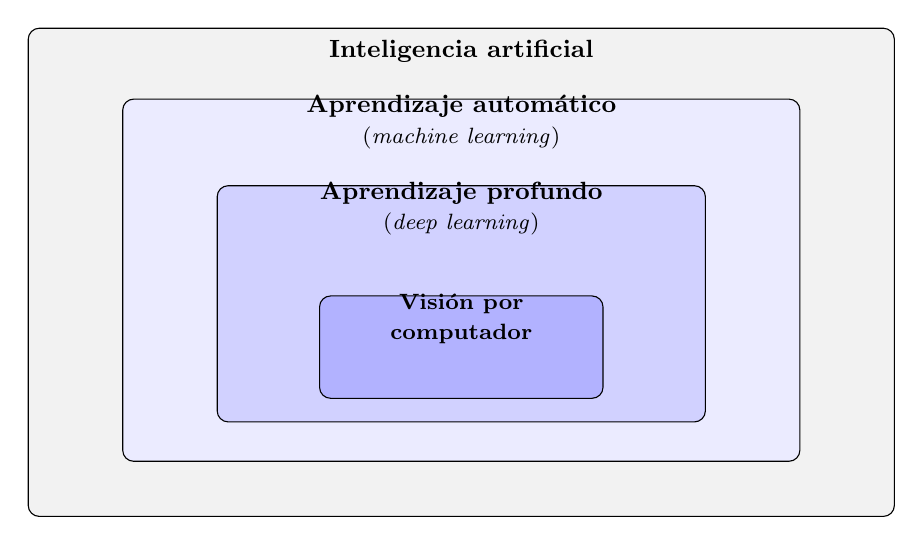
\begin{tikzpicture}[
  every node/.style={align=center, font=\small},
  box/.style={draw, rounded corners, minimum height=1.4cm}
]
\node[box, fill=gray!10, minimum width=11cm, minimum height=6.2cm, anchor=north] (ia) at (0,3) {};
\node[align=center] at (0,2.7) {\textbf{Inteligencia artificial}};
\node[box, fill=blue!8, minimum width=8.6cm, minimum height=4.6cm, anchor=north] (ml) at (0,2.1) {};
\node[align=center] at (0,1.8) {\textbf{Aprendizaje automático}\\\footnotesize{(\emph{machine learning})}};
\node[box, fill=blue!18, minimum width=6.2cm, minimum height=3.0cm, anchor=north] (dl) at (0,1.0) {};
\node[align=center] at (0,0.7) {\textbf{Aprendizaje profundo}\\\footnotesize{(\emph{deep learning})}};
\node[box, fill=blue!30, minimum width=3.6cm, minimum height=1.3cm, anchor=north] (cv) at (0,-0.4) {};
\node[align=center] at (0,-0.7) {\footnotesize\textbf{Visión por}\\\footnotesize\textbf{computador}};
\end{tikzpicture}
\caption{Relación de contención entre inteligencia artificial, aprendizaje
automático, aprendizaje profundo y visión por computador. La visión por
computador se apoya hoy predominantemente en aprendizaje profundo, aunque
históricamente incluye también técnicas no basadas en redes neuronales
(por ejemplo, K-means, sección~\ref{sec:fundamentos-kmeans}).}
\label{fig:jerarquia-ia}
\end{figure}

El \textbf{análisis de datos} es, en paralelo, la disciplina que convierte
datos generados por sensores o, como en este proyecto,
algoritmos de visión por computador, en información interpretable: medias,
distribuciones, mapas de calor, tendencias o comparativas
\citep{coursera2026dataanalysis}. La intersección
de ambos campos es precisamente lo que estructura este proyecto: primero se
usa visión por computador para producir datos de trayectorias a partir de
vídeo (capítulos~\ref{cap:diseno} y~\ref{cap:implementacion}), y después se
aplica análisis de datos sobre esas trayectorias para obtener metadatos
deportivos interpretables (mapas de calor, distancias, posesión), como se
detalla en la sección~\ref{sec:implementacion-metadatos}.

\section{Datasets y el ecosistema SoccerNet}
\label{sec:fundamentos-dataset}

Todo sistema de aprendizaje automático necesita datos con los que aprender
y, sobre todo, con los que poder evaluarse de forma objetiva. Un
\textbf{dataset} (conjunto de datos) es, en este contexto, una colección
organizada de ejemplos (en visión por computador, típicamente imágenes o
vídeos) acompañados de anotaciones de referencia (\emph{ground truth}) que
indican cuál es la respuesta correcta para cada ejemplo
\citep{ibm2026dataset}. Un
\textbf{benchmark} es, además, un dataset acompañado de un protocolo de
evaluación estandarizado (qué métricas se calculan, cómo se dividen los
datos en entrenamiento y test) que permite comparar de forma justa los
resultados obtenidos por distintos investigadores o equipos, incluso años
después y sin que hayan trabajado nunca juntos. Sin datasets públicos con
estas características, cualquier comparación entre algoritmos, como la que
constituye el núcleo de este proyecto, carecería de validez: cada autor
podría estar evaluando sobre datos distintos, más favorables a su propio
método. MOTChallenge \citep{motchallengeweb2026} y el propio
SoccerNet-Tracking \citep{cioppa2022soccernettracking}, presentados a
continuación, son dos ejemplos concretos de este tipo de benchmark
aplicados al seguimiento multiobjeto.

\textbf{SoccerNet} \citep{soccernetweb2026} es un
ecosistema de datasets y competiciones académicas anuales centrado en el
análisis automático de vídeo de fútbol profesional, mantenido por un
consorcio de investigadores de varias universidades. Ofrece múltiples
tareas sobre el mismo conjunto de partidos de origen (reconocimiento de
acciones, segmentación del tipo de plano de cámara, reconocimiento del
dorsal del jugador, seguimiento multiobjeto, entre otras), cada una con su
propio subconjunto de datos, su propio formato de anotación y su propio
protocolo de evaluación. La sección~\ref{sec:analisis-decision} del
capítulo~\ref{cap:analisis} detalla el proceso de exploración de estas
tareas alternativas antes de decidirse por la tarea de tracking.

\subsection{SoccerNet-Tracking}
\label{subsec:fundamentos-soccernet-tracking}

Este proyecto se apoya específicamente en \textbf{SoccerNet-Tracking}
\citep{cioppa2022soccernettracking}, la tarea de seguimiento multiobjeto del
ecosistema SoccerNet. El dataset está compuesto por 200 secuencias de vídeo
de 30 segundos cada una, extraídas de partidos profesionales reales y
seleccionadas por representar situaciones de juego especialmente exigentes
para el tracking (aglomeraciones de jugadores, cambios bruscos de
dirección, oclusiones). Cada secuencia se distribuye ya descompuesta en
frames individuales (formato de imagen), en lugar de como un fichero de
vídeo, lo que facilita el procesamiento frame a frame que exigen los
algoritmos de tracking.

\begin{figure}[htp]
\centering
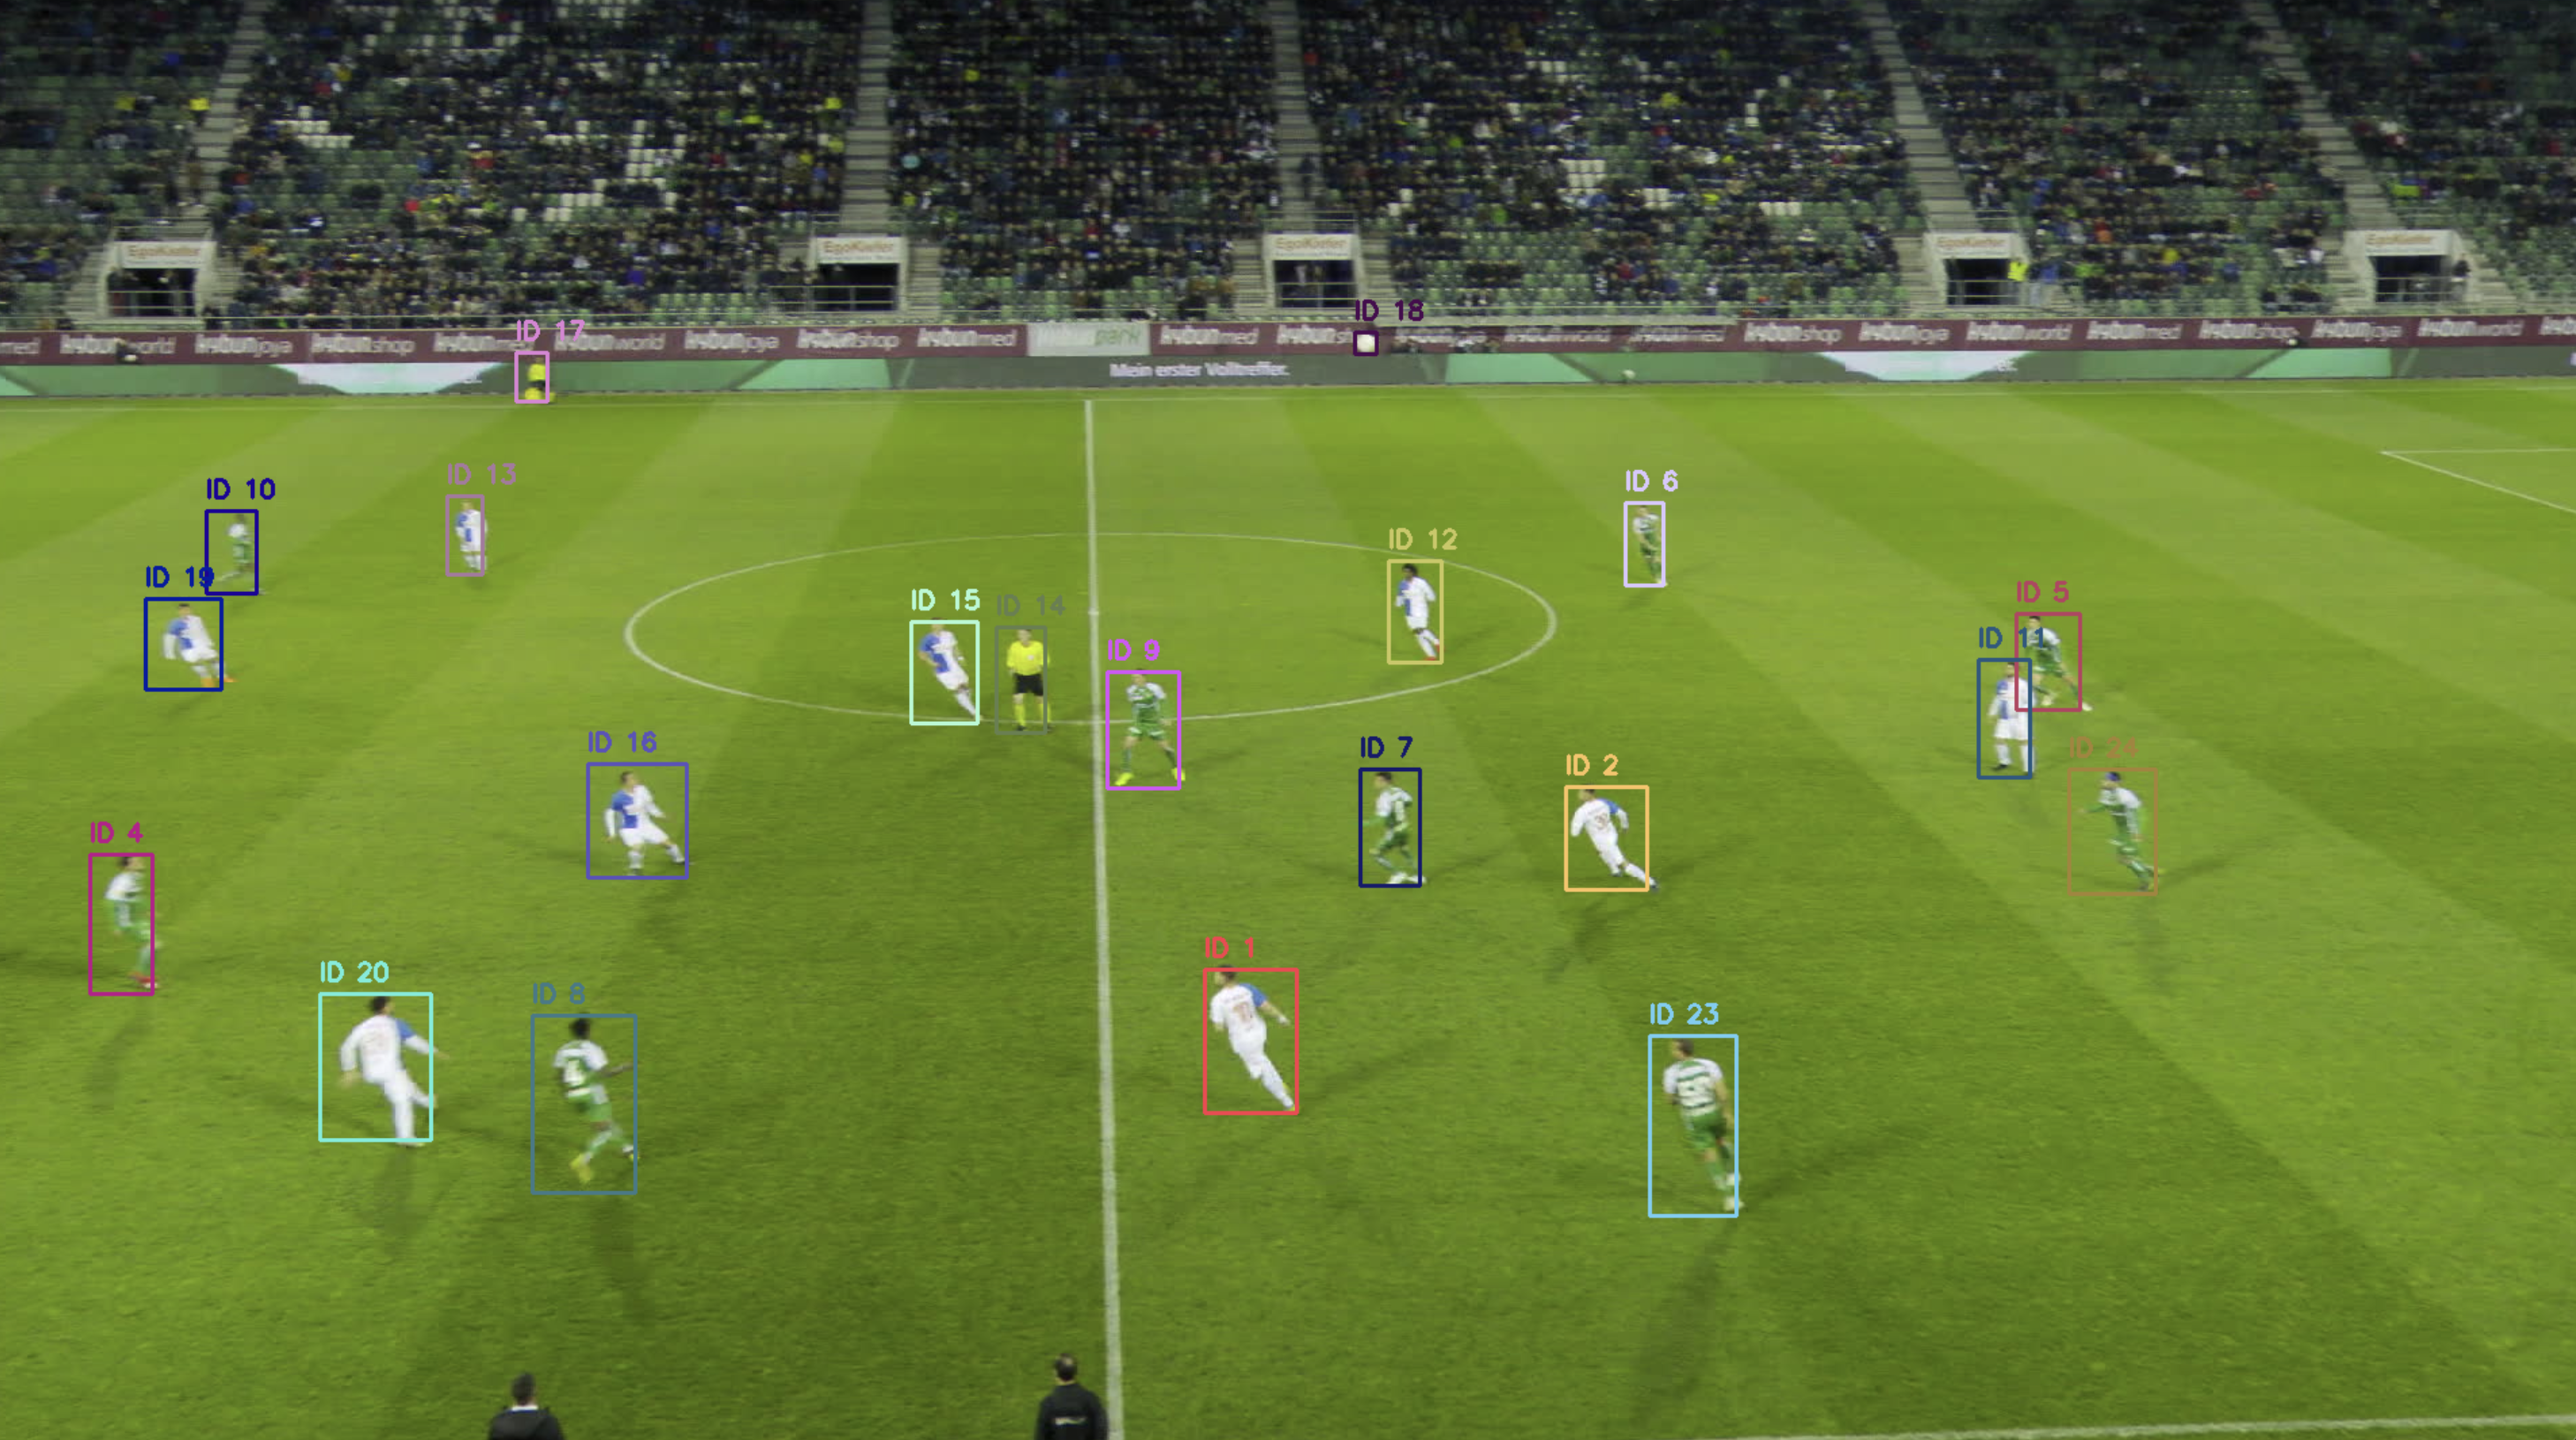
\includegraphics[width=0.92\textwidth]{figures/tracking-example.png}
\caption{Frame de una secuencia de SoccerNet-Tracking, con las cajas
delimitadoras y los identificadores de un resultado de tracking
superpuestos.}
\label{fig:tracking-example}
\end{figure}

Cada secuencia incluye, junto con los frames, los siguientes ficheros:

\begin{itemize}
  \item \textbf{\texttt{img1/}}: carpeta con los frames individuales de la
        secuencia, numerados de forma correlativa.
  \item \textbf{\texttt{det/det.txt}}: detecciones \emph{precomputadas} de
        cada objeto (jugadores, árbitros y balón) en cada frame, obtenidas
        con un detector de objetos ya entrenado por los organizadores del
        dataset. Esta es la entrada real de los algoritmos de tracking
        evaluados en este proyecto, como se explica en la
        sección~\ref{sec:fundamentos-mot}.
  \item \textbf{\texttt{gt/gt.txt}}: la posición e identidad
        \emph{real} de cada objeto en cada frame, usada como referencia
        para calcular las métricas de evaluación de la
        sección~\ref{sec:fundamentos-metricas}.
  \item \textbf{\texttt{seqinfo.ini}} y \textbf{\texttt{gameinfo.ini}}:
        metadatos de la secuencia (resolución de imagen, \emph{frame rate})
        y del partido de origen.
\end{itemize}

Tanto \texttt{det.txt} como \texttt{gt.txt} siguen el formato estándar del
protocolo \textbf{MOTChallenge} \citep{motchallengeweb2026},
el benchmark de referencia histórico en seguimiento multiobjeto (orientado
originalmente a vigilancia urbana de peatones, no a deporte), que
SoccerNet-Tracking reutiliza para que las herramientas de evaluación ya
existentes (en particular \texttt{TrackEval}, empleada en este proyecto
(sección~\ref{sec:implementacion-evaluacion})) funcionen sin
modificaciones. Cada línea de estos ficheros describe un objeto en un frame
concreto:

\begin{center}
\texttt{frame\_id, obj\_id, x, y, w, h, confianza, -1, -1, -1}
\end{center}

donde \texttt{frame\_id} identifica el frame, \texttt{obj\_id} identifica
al objeto (en \texttt{gt.txt}, su identidad real y consistente a lo largo
de toda la secuencia; en \texttt{det.txt}, este campo no se usa), y
\texttt{x, y, w, h} describen la posición y el tamaño de la caja
delimitadora (\emph{bounding box}) del objeto en píxeles, con
\texttt{(x, y)} la esquina superior izquierda. Los tres últimos campos,
fijos a \texttt{-1}, corresponden a información adicional (clase de objeto,
visibilidad) que MOTChallenge contempla para otros dominios pero que
SoccerNet-Tracking no utiliza.

El dataset se organiza en tres particiones o splits: un conjunto de
\textbf{entrenamiento} (57 secuencias, con gt.txt disponible,
usado para desarrollar y ajustar los algoritmos), un conjunto de
\textbf{test} (con gt.txt disponible, reservado para la evaluación
final y no consultado durante el ajuste, tal y como exige una evaluación
honesta) y un conjunto de \emph{\textbf{challenge}} (sin gt.txt,
usado únicamente para el ranking oficial de la competición SoccerNet, no utilizado
 en este proyecto).

\section{El problema del seguimiento multiobjeto}
\label{sec:fundamentos-mot}

El \textbf{seguimiento multiobjeto} (\emph{Multi-Object Tracking}, MOT)
consiste en asignar, a cada objeto de interés que aparece en un vídeo, una
identidad numérica que se mantenga consistente a lo largo de todos los
frames en los que ese objeto sea visible incluso si desaparece
temporalmente de la imagen, por ejemplo al quedar oculto detrás de otro
jugador, y reaparece poco después \citep{ultralytics2026track}. Un sistema de MOT completo resuelve,
en general, dos subproblemas relacionados pero conceptualmente distintos,
representados en la Figura~\ref{fig:fundamentos-mot-pipeline}:

\begin{enumerate}
  \item \textbf{Detección}: localizar dónde está cada objeto de interés en
        cada frame individual, sin ninguna noción de continuidad temporal,
        es decir, sin saber todavía si el objeto detectado en el frame
        $t$ es el mismo que se detectó en el frame $t-1$. Esta tarea se
        resuelve habitualmente con un detector de objetos entrenado con
        aprendizaje profundo (por ejemplo, la familia YOLO, discutida en la
        sección~\ref{subsec:fundamentos-balon}).
  \item \textbf{Asociación}: dado el conjunto de detecciones de cada frame,
        decidir qué detección del frame actual corresponde a qué identidad
        ya existente de frames anteriores, o si se trata de un objeto que
        aparece por primera vez. Este es el problema que resuelven
        específicamente los algoritmos de tracking comparados en este
        proyecto (sección~\ref{sec:fundamentos-algoritmos}).
\end{enumerate}

\begin{figure}[htp]
\centering
\begin{tikzpicture}[
  every node/.style={align=center, font=\small},
  box/.style={draw, rounded corners, fill=blue!10, minimum width=2.6cm, minimum height=1.1cm},
  arrow/.style={-{Latex[length=2.5mm]}, thick}
]
\node[box] (frame) {Frame de vídeo};
\node[box, right=1.4cm of frame] (det) {Detección\\\footnotesize{(dónde está)}};
\node[box, right=1.4cm of det] (asoc) {Asociación\\\footnotesize{(quién es)}};
\node[box, right=1.4cm of asoc] (id) {Identidades\\consistentes};
\draw[arrow] (frame) -- (det);
\draw[arrow] (det) -- (asoc);
\draw[arrow] (asoc) -- (id);
\node[align=center, font=\footnotesize] at ($(det)!0.5!(asoc) + (0,-1.3)$)
  {Este proyecto se centra únicamente en la asociación.};
\end{tikzpicture}
\caption{Las dos etapas de un sistema de MOT: detección y asociación.}
\label{fig:fundamentos-mot-pipeline}
\end{figure}

Como se explicó en la sección~\ref{sec:intro-problema}, este proyecto se
sitúa solo en la segunda mitad de ese proceso: dado que
SoccerNet-Tracking proporciona las detecciones ya calculadas en
\texttt{det.txt} (sección~\ref{subsec:fundamentos-soccernet-tracking}), la
tarea abordada es específicamente la asociación, también llamada
\emph{tracking-by-detection} en la literatura, por oposición a los métodos
de \emph{joint detection and tracking} que entrenan un único modelo capaz
de detectar y asociar a la vez. Esta decisión, natural dado el
planteamiento del dataset, es también la que sigue la comparativa oficial
de SoccerNet-Tracking, lo que permite que los resultados de este proyecto
sean comparables con los de otros participantes de la competición.

\subsection{Retos específicos del seguimiento en fútbol}

El fútbol es un escenario particularmente exigente para el MOT, mucho más
que los entornos de vigilancia urbana o conducción autónoma para los que
originalmente se diseñaron muchos de los algoritmos clásicos del campo,
hoy ampliamente aplicados en escenarios reales de ese tipo
\citep{ultralytics2026track}. Entre los factores que lo hacen especialmente
difícil:

\begin{itemize}
  \item \textbf{Número elevado y constante de objetos}: veintidós
        jugadores, uno o varios árbitros y el balón se mueven de forma
        simultánea durante todo el partido, frente a los escenarios más
        dispersos de la vigilancia urbana.
  \item \textbf{Apariencia muy similar entre objetos}: los jugadores de un
        mismo equipo visten la misma camiseta, lo que hace que los métodos
        de asociación basados en apariencia visual (re-identificación,
        sección~\ref{subsec:fundamentos-reid}) sean menos discriminativos
        que en otros dominios, donde cada persona suele vestir de forma
        distinta.
  \item \textbf{Oclusiones frecuentes}: los jugadores se cruzan y agrupan
        constantemente (disputas de balón, saques de esquina, barreras en
        faltas), lo que provoca oclusiones parciales o totales que ponen a
        prueba la capacidad de un algoritmo de mantener la identidad de un
        jugador mientras está oculto y de recuperarla correctamente al
        reaparecer.
  \item \textbf{Movimiento no lineal}: a diferencia de un peatón o un
        vehículo, que en general mantienen una trayectoria relativamente
        predecible durante fracciones de segundo, un jugador de fútbol
        puede cambiar de dirección y de velocidad de forma muy brusca (un
        regate, una parada súbita), lo que penaliza a los modelos de
        movimiento más simples, como se discute en la
        sección~\ref{subsec:fundamentos-ocsort}.
  \item \textbf{El balón como caso extremo}: al margen de las personas, el
        balón es un objeto pequeño, de movimiento muy rápido y no lineal
        (rebotes, golpeos), y visualmente casi indistinguible de otros
        elementos redondeados y claros del campo. La sección
        \ref{subsec:fundamentos-balon} detalla cómo se ha abordado su detección en este proyecto.
\end{itemize}

\section{Fundamentos de \emph{tracking-by-detection}}
\label{sec:fundamentos-tbd}

Antes de describir los algoritmos concretos comparados en este proyecto
(sección~\ref{sec:fundamentos-algoritmos}), conviene introducir los dos
bloques matemáticos sobre los que se construyen prácticamente todos los
métodos clásicos de \emph{tracking-by-detection}: un modelo que predice
dónde estará cada objeto en el siguiente frame, y un procedimiento que
decide qué detección real se asocia a cada predicción.

\subsection{El filtro de Kalman}
\label{subsec:fundamentos-kalman}

El \textbf{filtro de Kalman} \citep{wikipedia2026kalman} es un algoritmo recursivo
que estima el estado de un sistema dinámico, en este caso, la posición y
la velocidad de un objeto que se mueve a partir de observaciones ruidosas
a lo largo del tiempo. Funciona mediante un ciclo de dos fases que se repite
en cada frame, representado en la Figura~\ref{fig:fases-filtro-kalman}:

\begin{enumerate}
  \item \textbf{Predicción}: a partir del estado estimado en el frame
        anterior (posición y velocidad), el filtro predice dónde debería
        estar el objeto en el frame actual, asumiendo un modelo de
        movimiento simple (típicamente, velocidad constante).
  \item \textbf{Corrección} (o actualización): cuando llega la observación
        real de ese frame en este caso, la detección que finalmente se le
        asocie mediante el procedimiento de la
        sección~\ref{subsec:fundamentos-hungaro}, el filtro combina esa
        observación con su propia predicción, ponderando cada una según su
        incertidumbre estimada, para obtener una estimación corregida del
        estado.
\end{enumerate}

\begin{figure}[htp]
\centering
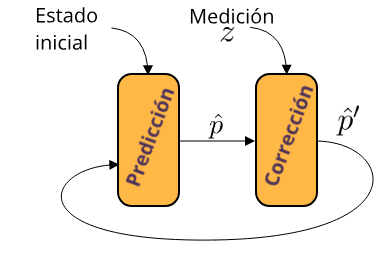
\includegraphics[width=0.5\textwidth]{figures/filtro_kalman.png}
\caption{Ciclo predicción-corrección del filtro de Kalman, repetido en cada frame para cada objeto seguido.}
\label{fig:fases-filtro-kalman}
\end{figure}

Este ciclo tiene una consecuencia práctica importante para el tracking: aun
cuando un objeto deja de detectarse durante varios frames (por ejemplo, por
una oclusión), el filtro de Kalman sigue pudiendo predecir su posición
probable basándose en su movimiento anterior, lo que permite mantener viva
su identidad y recuperar la asociación correcta cuando vuelve a detectarse.
Los tres algoritmos comparados y considerados en este proyecto (SORT,
OC-SORT y ByteTrack, sección~\ref{sec:fundamentos-algoritmos}) usan
variantes de un filtro de Kalman como modelo de movimiento subyacente.

\subsection{Solapamiento entre cajas: IoU}
\label{subsec:fundamentos-iou}

Para decidir si una detección de un frame corresponde al mismo objeto que
una predicción de Kalman (o que otra detección de un frame anterior), los
métodos de \emph{tracking-by-detection} necesitan una medida de similitud
entre dos cajas delimitadoras. La más utilizada, por su simplicidad y bajo
coste computacional, es la \textbf{Intersección sobre Unión} (\emph{Intersection
over Union}, IoU): dadas dos cajas $A$ y $B$, se define como

\begin{equation}
\mathrm{IoU}(A, B) = \frac{|A \cap B|}{|A \cup B|},
\label{eq:fundamentos-iou}
\end{equation}

es decir, el área de la región donde ambas cajas se solapan, dividida entre
el área total que cubren entre las dos. La IoU vale 1 cuando las cajas
coinciden exactamente y 0 cuando no se solapan en absoluto, lo que la hace
directamente interpretable como un porcentaje de acuerdo espacial (véase la
Figura~\ref{fig:fundamentos-iou}).

\begin{figure}[htp]
\centering
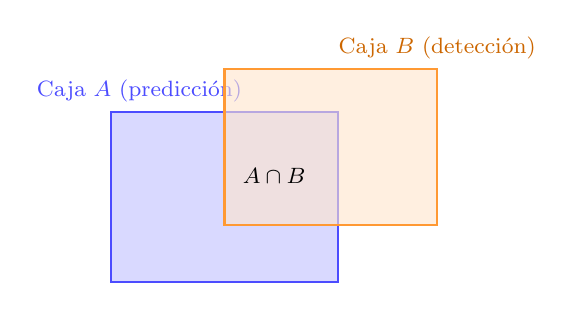
\begin{tikzpicture}[scale=0.9]
\draw[fill=blue!15, draw=blue!70, thick] (0,0) rectangle (3.2,2.4);
\node[blue!70] at (0.4,2.7) {\footnotesize Caja $A$ (predicción)};
\draw[fill=orange!20, draw=orange!80, thick, fill opacity=0.6] (1.6,0.8) rectangle (4.6,3.0);
\node[orange!80!black] at (4.6,3.3) {\footnotesize Caja $B$ (detección)};
\node[font=\footnotesize] at (2.3,1.5) {$A \cap B$};
\end{tikzpicture}
\caption{Intersección sobre Unión (IoU) entre una caja predicha por Kalman
(A) y una detección real (B): la región sombreada de solape, dividida entre
el área total ocupada por ambas cajas.}
\label{fig:fundamentos-iou}
\end{figure}

\subsection{El problema de asignación y el algoritmo húngaro}
\label{subsec:fundamentos-hungaro}

Una vez calculada una matriz de similitud (por ejemplo, de IoU) entre todas
las predicciones activas y todas las detecciones de un frame, queda por
resolver el \textbf{problema de asignación}: encontrar la correspondencia
uno a uno entre predicciones y detecciones que maximice la similitud total,
sin que ninguna detección se asocie a más de una predicción ni viceversa.
Resolver este problema por fuerza bruta (probar todas las combinaciones
posibles) tiene un coste factorial en el número de objetos, inviable ya
con unas pocas decenas de jugadores en pantalla.

El \textbf{algoritmo húngaro} \citep{wikipedia2026hungaro} resuelve este
problema de forma exacta y en tiempo polinómico. Dada una matriz de coste
$M$ (que puede construirse, por ejemplo, como $1 - \mathrm{IoU}$, de modo
que minimizar coste equivale a maximizar solapamiento), el algoritmo
encuentra la asignación completa de coste mínimo mediante una serie de
transformaciones de la matriz que no alteran la asignación óptima pero
reducen progresivamente el problema, hasta poder leer la solución
directamente. En la práctica, ninguno de los algoritmos de tracking usados
en este proyecto implementa el algoritmo húngaro desde cero: todos delegan
en la implementación ya optimizada de \texttt{scipy} o de librerías
equivalentes, a través de la librería \texttt{boxmot} descrita en la
sección~\ref{sec:implementacion-entorno}.

Un detalle que puede ser importante a la hora de entender ByteTrack en la
sección~\ref{subsec:fundamentos-bytetrack} es que no toda asignación con
coste finito se acepta: se suele imponer un umbral mínimo de similitud
(por ejemplo, IoU mínima) por debajo del cual una predicción y una detección no
se consideran candidatas a asociarse, aunque el algoritmo húngaro las
hubiera emparejado matemáticamente. Las predicciones que no encuentran
ninguna detección compatible se marcan como no observadas en ese frame
, mientras que las
detecciones que no encuentran ninguna predicción compatible inician una
identidad nueva.

\section{Algoritmos de tracking comparados}
\label{sec:fundamentos-algoritmos}

Con los fundamentos de las secciones anteriores, esta sección describe los
dos algoritmos efectivamente implementados y comparados en este proyecto
ByteTrack y OC-SORT así como el algoritmo histórico del que ambos
derivan (SORT) y las familias de algoritmos que se consideraron pero
finalmente no se implementaron, con la justificación de por qué.

\subsection{SORT: el punto de partida}
\label{subsec:fundamentos-sort}

\textbf{SORT} (\emph{Simple Online and Realtime Tracking},
\citealp{bewley2016sort, ultralytics2026trackingtools}) es el algoritmo que sentó las bases del
\emph{tracking-by-detection} moderno: para cada objeto seguido, mantiene un
filtro de Kalman (sección~\ref{subsec:fundamentos-kalman}) que predice su
posición en el frame actual; calcula la IoU (sección~\ref{subsec:fundamentos-iou})
entre esas predicciones y todas las detecciones del frame; resuelve la
asignación óptima con el algoritmo húngaro
(sección~\ref{subsec:fundamentos-hungaro}); y actualiza cada filtro de
Kalman con la detección que le ha correspondido. Su principal virtud, que
explica su influencia posterior, es la simplicidad: no requiere ningún
modelo de apariencia visual ni entrenamiento adicional más allá del propio
detector de objetos, lo que lo hace extremadamente rápido.

SORT tiene, sin embargo, una limitación conocida que motivó buena parte de
las mejoras posteriores: solo considera para la asociación las detecciones
de \emph{alta confianza} del detector, descartando directamente las de
confianza intermedia o baja. En escenarios con oclusiones frecuentes como
el fútbol, un jugador parcialmente ocluido suele generar una detección de
confianza más baja (o directamente no generar ninguna), lo que provoca que
SORT pierda su identidad con más facilidad de la deseable y genere más
\emph{cambios de identidad} (\emph{ID switches}) de los necesarios. Esta
limitación es precisamente la que aborda ByteTrack.

En \texttt{boxmot}, la librería usada en este proyecto
(sección~\ref{sec:implementacion-entorno}), no existe una implementación
del SORT original independiente: la clase disponible más próxima es
\texttt{OCSORT}, su evolución directa descrita en la
sección~\ref{subsec:fundamentos-ocsort}. Por ese motivo, y como se explica
en el capítulo~\ref{cap:implementacion}, el script de este proyecto que
originalmente pretendía implementar SORT (\texttt{sort\_alg.py}) contiene en
realidad OC-SORT, quedando el nombre del fichero como huella de
esa decisión.

\subsection{OC-SORT: SORT centrado en la observación}
\label{subsec:fundamentos-ocsort}

\textbf{OC-SORT} (\emph{Observation-Centric SORT}, \citealp{cao2023ocsort})
identifica y corrige dos problemas concretos de SORT, sin abandonar su
simplicidad y velocidad. El primero es lo que sus autores llaman
\emph{acumulación de error durante la desaparición}: cuando un objeto deja
de detectarse durante varios frames (oclusión), el filtro de Kalman de
SORT sigue extrapolando su posición usando exclusivamente su propio modelo
de movimiento, sin ninguna corrección, de modo que el error de la
predicción crece sin control cuanto más dura la oclusión; al reaparecer el
objeto, la predicción puede estar ya demasiado lejos de la posición real
para una asociación correcta. El segundo es la sensibilidad del filtro de
Kalman a los movimientos no lineales,
especialmente marcados en fútbol.

OC-SORT resuelve ambos problemas centrando el filtro en las
\emph{observaciones reales} en lugar de en el estado interno acumulado por
Kalman: en lugar de corregir el filtro paso a paso con predicciones
intermedias durante toda la desaparición, cuando el objeto reaparece
OC-SORT recalcula directamente su trayectoria a partir de la última
observación real conocida antes de desaparecer y la primera observación
real al reaparecer, evitando así la deriva acumulada. Este enfoque, más
robusto ante oclusiones largas y movimientos bruscos, es el que motivó su
inclusión en la comparativa de este proyecto junto con ByteTrack.

\subsection{ByteTrack: aprovechar todas las detecciones}
\label{subsec:fundamentos-bytetrack}

\textbf{ByteTrack} \citep{zhang2022bytetrack, ultralytics2026trackingtools} aborda directamente la
limitación de SORT descrita en la sección~\ref{subsec:fundamentos-sort}: en
lugar de descartar las detecciones de baja confianza, las aprovecha en una
\emph{segunda ronda} de asociación. Su procedimiento, para cada frame, es
el siguiente:

\begin{enumerate}
  \item Se separan las detecciones del frame en dos grupos según un umbral
        de confianza: de \textbf{alta} y de \textbf{baja} confianza.
  \item \textbf{Primera asociación}: se emparejan las predicciones de
        Kalman con las detecciones de alta confianza, con el procedimiento
        estándar de IoU y algoritmo húngaro
        (secciones~\ref{subsec:fundamentos-iou}
        y~\ref{subsec:fundamentos-hungaro}).
  \item \textbf{Segunda asociación}: las predicciones que no encontraron
        pareja en el paso anterior normalmente son objetos parcialmente
        ocluidos cuya detección, si existe, es de baja confianza. Estas
        predicciones se intentan emparejar de nuevo, esta vez únicamente contra las
        detecciones de baja confianza.
  \item Las predicciones que siguen sin pareja tras ambas rondas se
        mantienen como activas sin observación (apoyándose en el filtro de
        Kalman) durante un número limitado de frames antes de eliminarse
        definitivamente y las detecciones de alta confianza que no
        encontraron ninguna predicción compatible inician identidades
        nuevas.
\end{enumerate}

\begin{figure}[htp]
\centering
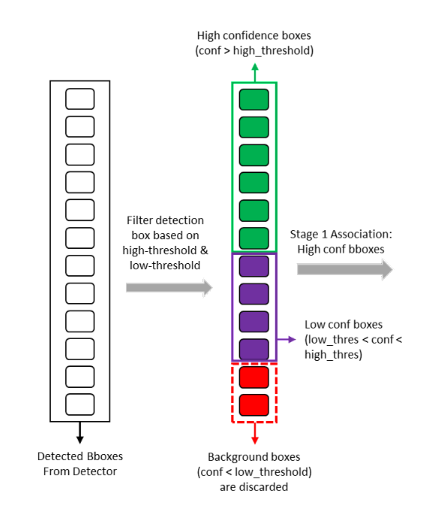
\includegraphics[width=0.7\textwidth]{figures/bytetrack-detec.png}
\caption{Las dos rondas de asociación de ByteTrack: primero con
detecciones de alta confianza, después con las de baja confianza,
recuperando así objetos parcialmente ocluidos que SORT descartaría
\citep{zhang2022bytetrack}.}
\label{fig:fundamentos-bytetrack}
\end{figure}

Esta segunda ronda es, precisamente, lo que hace a ByteTrack especialmente
adecuado para el fútbol: un jugador ocluido detrás de otro suele seguir
generando una detección débil (de baja confianza) en lugar de ninguna
detección, y ByteTrack es capaz de aprovechar esa señal parcial en lugar de
descartarla, a diferencia de SORT y, en menor medida, de OC-SORT.

\subsection{Trackers con re-identificación visual: considerados y no implementados}
\label{subsec:fundamentos-reid}

Los tres algoritmos descritos hasta ahora (SORT, OC-SORT, ByteTrack)
pertenecen a la familia de trackers \emph{sin apariencia}: solo usan la
posición y el tamaño de las cajas delimitadoras para asociar, nunca el
aspecto visual del objeto. Existe una familia paralela de algoritmos que
incorpora, además, un modelo de \textbf{re-identificación} (\emph{Re-ID}):
una red neuronal, entrenada por separado, que extrae un vector numérico
(\emph{embedding}) representativo de la apariencia visual de cada objeto,
de modo que dos detecciones del mismo objeto puedan reconocerse por similitud de
apariencia y no solo por proximidad espacial. \textbf{DeepSORT}
\citep{wojke2017deepsort, ultralytics2026trackingtools} fue el primer algoritmo relevante en incorporar
esta idea sobre la base de SORT, y su enfoque se ha extendido después a
variantes más recientes como StrongSORT o BoT-SORT, todas ellas también
disponibles en \texttt{boxmot}.

El tutor de este proyecto planteó explícitamente, en una de las reuniones
de seguimiento (sección~\ref{sec:gestion-roles}), la posibilidad de ampliar
la comparativa con algoritmos de esta familia. Finalmente no se ha
incorporado ningún tracker con Re-ID a este proyecto, por dos motivos
principales. En primer lugar, una comparación justa exigiría fijar el mismo
modelo de Re-ID para todos los algoritmos comparados (por ejemplo,
\texttt{osnet\_x0\_25\_msmt17}, disponible directamente en
\texttt{boxmot}), lo que añade una variable más --la calidad del propio
modelo de Re-ID, no entrenado por el equipo del proyecto ni específico de
fútbol-- a una comparativa que, sin esa variable, ya resultaba
suficientemente rica con el estudio de hiperparámetros de los dos
algoritmos sin apariencia (capítulo~\ref{cap:implementacion}). En segundo
lugar, como se ha señalado en la sección~\ref{sec:fundamentos-mot}, la
apariencia visual es un criterio especialmente poco discriminativo en
fútbol (los compañeros de equipo visten de forma prácticamente idéntica),
lo que hace previsible que el margen de mejora aportado por Re-ID en este
dominio concreto sea menor que en otros escenarios de MOT donde cada
persona viste de forma distinta.

\section{Métricas de evaluación de sistemas de tracking}
\label{sec:fundamentos-metricas}

Comparar dos algoritmos de tracking exige una forma objetiva de medir su
rendimiento sobre el \emph{ground truth} (\texttt{gt.txt},
sección~\ref{subsec:fundamentos-soccernet-tracking}). Esta sección presenta
las tres familias de métricas empleadas en este proyecto y calculadas con
\texttt{TrackEval} (sección~\ref{sec:implementacion-evaluacion}): MOTA/MOTP
(las más clásicas), IDF1 (centrada en la consistencia de identidad) y HOTA
(la más reciente y equilibrada, adoptada como métrica principal de este
proyecto).

\subsection{CLEAR MOT: MOTA y MOTP}

Las métricas \textbf{CLEAR MOT} \citep{bernardin2008clearmot} fueron,
durante más de una década, el estándar de facto en la evaluación de
sistemas de tracking. \textbf{MOTA} (\emph{Multiple Object Tracking
Accuracy}) resume en un único porcentaje tres tipos de error acumulados a
lo largo de toda la secuencia: falsos negativos (objetos reales no
detectados), falsos positivos (detecciones que no corresponden a ningún
objeto real) y cambios de identidad (\emph{ID switches}, cuando el
algoritmo confunde la identidad de un objeto con la de otro). \textbf{MOTP}
(\emph{Multiple Object Tracking Precision}), complementaria a MOTA, mide la
precisión espacial media de las cajas correctamente emparejadas (cuánto se
solapan, en promedio, con el \emph{ground truth}), sin penalizar los
errores de asociación que ya recoge MOTA.

La principal limitación de MOTA, señalada posteriormente varias veces
en este documento \citep{luiten2021hota}, es que pondera con mucho más peso los
errores de detección (falsos positivos y negativos) que los errores de
asociación (cambios de identidad): un algoritmo puede detectar
correctamente a casi todos los jugadores en casi todos los frames y aun así
confundir sistemáticamente sus identidades, obteniendo una MOTA
engañosamente alta pese a ser, en la práctica, poco útil para cualquier
análisis que dependa de trayectorias individuales consistentes, como el
pipeline de metadatos de este mismo proyecto
(sección~\ref{sec:implementacion-metadatos}).

\subsection{IDF1}

\textbf{IDF1} \citep{ristani2016idf1} nace precisamente para corregir ese
desequilibrio, centrando la evaluación en la consistencia de identidad en
lugar de en la detección frame a frame. Se calcula como la media armónica
(F1) entre la precisión y la exhaustividad (\emph{recall}) de identidad,
calculadas tras resolver una única asignación óptima,de nuevo mediante el
algoritmo húngaro, sección~\ref{subsec:fundamentos-hungaro} entre las
trayectorias predichas por el algoritmo y las trayectorias reales del
\emph{ground truth} a lo largo de \emph{toda} la secuencia, no frame a
frame. En la práctica, IDF1 penaliza con mucha más severidad que MOTA los
cambios de identidad, y es una de las tres métricas reportadas en los
resultados de este proyecto (capítulo~\ref{cap:pruebas}).

\subsection{HOTA: la métrica principal de este proyecto}
\label{subsec:fundamentos-hota}

\textbf{HOTA} (\emph{Higher Order Tracking Accuracy},
\citealp{luiten2021hota, luiten2021hotablog}) es la métrica más reciente de las tres, propuesta
explícitamente para resolver el desequilibrio entre detección y asociación
que arrastraban tanto MOTA (sesgada hacia la detección) como IDF1 (sesgada
hacia la asociación). HOTA se define como la media geométrica de dos
componentes independientes:

\begin{equation}
\mathrm{HOTA} = \sqrt{\mathrm{DetA} \times \mathrm{AssA}},
\label{eq:fundamentos-hota}
\end{equation}

donde \textbf{DetA} (\emph{Detection Accuracy}) mide, de forma análoga a
MOTA, qué tan bien se detectan los objetos, y \textbf{AssA}
(\emph{Association Accuracy}) mide, de forma análoga a IDF1, qué tan bien
se mantienen las identidades a lo largo del tiempo. Al tomar la media
geométrica en lugar de una suma ponderada, HOTA exige que un algoritmo sea
bueno en ambos aspectos simultáneamente: un valor muy alto en uno de
los dos componentes no puede compensar un valor muy bajo en el otro, a
diferencia de lo que ocurriría con una media aritmética.

Una particularidad adicional de HOTA, relevante para la interpretación de
los resultados de este proyecto (capítulo~\ref{cap:pruebas}), es que ambos
componentes se calculan y promedian sobre un rango de umbrales de
solapamiento IoU, en lugar
de sobre un único umbral fijo como hacen MOTA e IDF1, que en TrackEval,
se calculan típicamente al 50\,\%
de IoU. Esta característica hace de HOTA una métrica más exigente y
completa, ya que resume el comportamiento del algoritmo tanto ante
exigencias de solapamiento laxas como estrictas, y es la razón por la que
se ha adoptado como métrica principal de comparación en este proyecto.

\section{Detección del balón}
\label{subsec:fundamentos-balon}

Aunque, como se ha explicado en la sección~\ref{sec:fundamentos-mot}, este
proyecto no aborda la detección de objetos (se parte de \texttt{det.txt}
ya calculado), existe un matiz importante: SoccerNet-Tracking incluye en
ese mismo fichero las detecciones del balón mezcladas con las de jugadores
y árbitros, sin distinguir explícitamente de qué tipo de objeto se trata
cada detección. Separar el balón del resto de objetos es, por tanto, un
paso de preprocesamiento necesario antes de aplicar cualquier algoritmo de
tracking, ya que el balón sigue una dinámica de movimiento completamente
distinta a la de una persona, es más rápido y con rebotes. Por tanto,
no tiene sentido
tratarlo con el mismo filtro de Kalman ni contarlo en las métricas de
tracking de personas.

La primera aproximación explorada para resolver este paso fue emplear un
detector de objetos entrenado con aprendizaje profundo, concretamente
\textbf{YOLO} (\emph{You Only Look Once}, \citealp{redmon2016yolo, ultralytics2026yolov8}) en su
versión ligera YOLOv8n, aplicado directamente sobre los frames para
localizar el balón de forma independiente al \texttt{det.txt} del dataset.
Este enfoque se descartó tras las primeras pruebas: el modelo, sin
reentrenar específicamente para balones de fútbol en las condiciones de
cámara e iluminación de las retransmisiones de SoccerNet, obtenía
resultados muy pobres, tanto falsos negativos (balón no detectado) como
falsos positivos sobre otros objetos redondeados y claros del campo, y
entrenarlo específicamente para esta única tarea auxiliar quedaba fuera del
alcance proporcional de este proyecto.

Se optó, en su lugar, por un \textbf{filtro geométrico} simple aplicado
directamente sobre las detecciones ya existentes en \texttt{det.txt}: una
detección se clasifica como balón si su área en píxeles es menor que un
umbral y su proporción ancho/alto es próxima a 1 (es decir, aproximadamente
cuadrada, coherente con la silueta de un balón visto desde prácticamente
cualquier ángulo), condiciones que rara vez cumple una persona. Este
filtro, con los umbrales exactos empleados, se detalla en la
sección~\ref{sec:implementacion-tracking} del
capítulo~\ref{cap:implementacion}; se trata de una heurística simple y con
limitaciones conocidas (puede confundir a un jugador muy lejano y pequeño
con el balón), pero suficiente para el propósito de excluir al balón del
tracking de personas sin necesidad de entrenar un modelo adicional.

\section{Clasificación no supervisada de jugadores por equipo: K-means y el árbitro}
\label{sec:fundamentos-kmeans}

Una vez obtenidas las trayectorias de los jugadores (capítulo~\ref{cap:implementacion}),
buena parte de los metadatos deportivos de interés como mapas de calor por
equipo, posesión por equipo (sección~\ref{sec:implementacion-metadatos})
requieren saber a qué equipo pertenece cada jugador. SoccerNet-Tracking no
proporciona esa información directamente, por lo que este proyecto la
infiere a partir del color dominante de la camiseta de cada jugador,
mediante \textbf{K-means}.

K-means \citep{ibm2026kmeans} es un algoritmo de \textbf{aprendizaje no
supervisado}: a diferencia de los algoritmos de aprendizaje supervisado que
aprenden a partir de ejemplos ya etiquetados con la respuesta correcta
(sección~\ref{sec:fundamentos-ia}), K-means agrupa datos sin ninguna
etiqueta previa, únicamente a partir de su similitud mutua. Dado un
conjunto de puntos (en este proyecto, colores representados como vectores
de tres componentes en el espacio BGR) y un número $k$ de grupos deseado,
el algoritmo procede de forma iterativa:

\begin{enumerate}
  \item Se inicializan $k$ centroides (puntos representativos de cada
        grupo), habitualmente de forma aleatoria o mediante alguna
        heurística de inicialización.
  \item \textbf{Asignación}: cada punto del conjunto de datos se asigna al
        centroide más cercano (típicamente, en distancia euclídea).
  \item \textbf{Actualización}: cada centroide se recalcula como la media
        de todos los puntos que se le han asignado.
  \item Los pasos 2 y 3 se repiten hasta que las asignaciones dejan de
        cambiar (convergencia) o se alcanza un número máximo de
        iteraciones.
\end{enumerate}

\begin{figure}[htp]
\centering
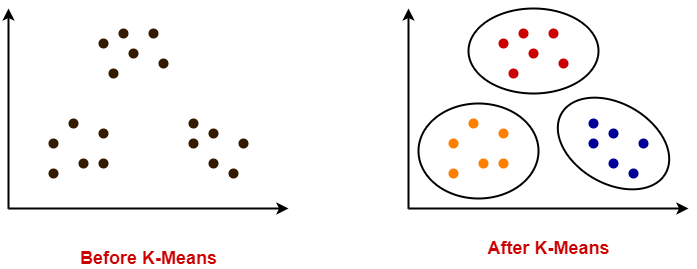
\includegraphics[width=0.85\textwidth]{figures/kmeans_before_after.png}
\caption{Efecto de K-means sobre un conjunto de puntos: antes del
agrupamiento (izquierda) y después de converger a $k=3$ grupos, cada uno
alrededor de su centroide (derecha) \citep{gatevidyalay2026kmeans}.}
\label{fig:fundamentos-kmeans-ejemplo}
\end{figure}

Formalmente, lo que este procedimiento iterativo minimiza es la suma de
las distancias euclídeas al cuadrado entre cada punto y el centroide de su
grupo \citep{ibm2026kmeans}:

\begin{equation}
\arg\min_{S} \sum_{i=1}^{k} \sum_{\mathbf{x} \in S_i} \lVert \mathbf{x} - \boldsymbol{\mu}_i \rVert^2,
\label{eq:fundamentos-kmeans}
\end{equation}

donde $S_i$ es el conjunto de puntos asignados al grupo $i$-ésimo y
$\boldsymbol{\mu}_i$ su centroide. El paso de \textbf{actualización} de
cada centroide como la media de sus puntos asignados es, precisamente, el
que reduce este error en cada iteración, hasta alcanzar un mínimo local.

En este proyecto, K-means se aplica en dos niveles, detallados con sus
parámetros concretos en la sección~\ref{sec:implementacion-metadatos}: primero,
con $k=1$, para extraer el color dominante de la camiseta de cada
detección individual de jugador (el color medio de una región recortada del
torso); después, con $k=2$ sobre el conjunto de todos esos colores
dominantes, asumiendo que existen exactamente dos equipos con colores de
camiseta distintos entre sí.

Esa asunción de $k=2$ es, precisamente, la limitación más relevante de este
enfoque y una de las cosas consideradas pero no resueltas en este proyecto:
el árbitro, con una camiseta de color distinto a la de ambos equipos, no
encaja en ninguno de los dos grupos y termina asignado por K-means al
centroide más próximo por color, es decir, a uno de los dos equipos de
forma incorrecta. Se valoró pero no se llegó a implementar una variante con
$k=3$ combinada con una heurística adicional (el grupo con menos
detecciones totales, dado que solo hay un árbitro principal frente a unos
once jugadores por equipo, se etiquetaría como árbitro en lugar de como
tercer equipo); esta mejora queda documentada como línea de trabajo futuro
en el capítulo~\ref{cap:conclusiones}.

\section{Homografía y proyección de coordenadas}
\label{sec:fundamentos-homografia}

Las posiciones de los jugadores que produce el tracking están expresadas en
\textbf{coordenadas de píxel} de la imagen de la cámara de retransmisión:
un sistema de referencia bidimensional propio de cada frame, sin relación
directa con las distancias reales sobre el terreno de juego. Para poder
calcular metadatos con sentido físico (distancia recorrida en metros,
velocidad en km/h, o simplemente representar las posiciones sobre un dibujo
del campo con proporciones correctas (sección~\ref{sec:implementacion-metadatos}))
es necesario transformar esas coordenadas de píxel a
\textbf{coordenadas reales del campo}, expresadas en metros sobre un plano
cenital.

\begin{figure}[htp]
\centering
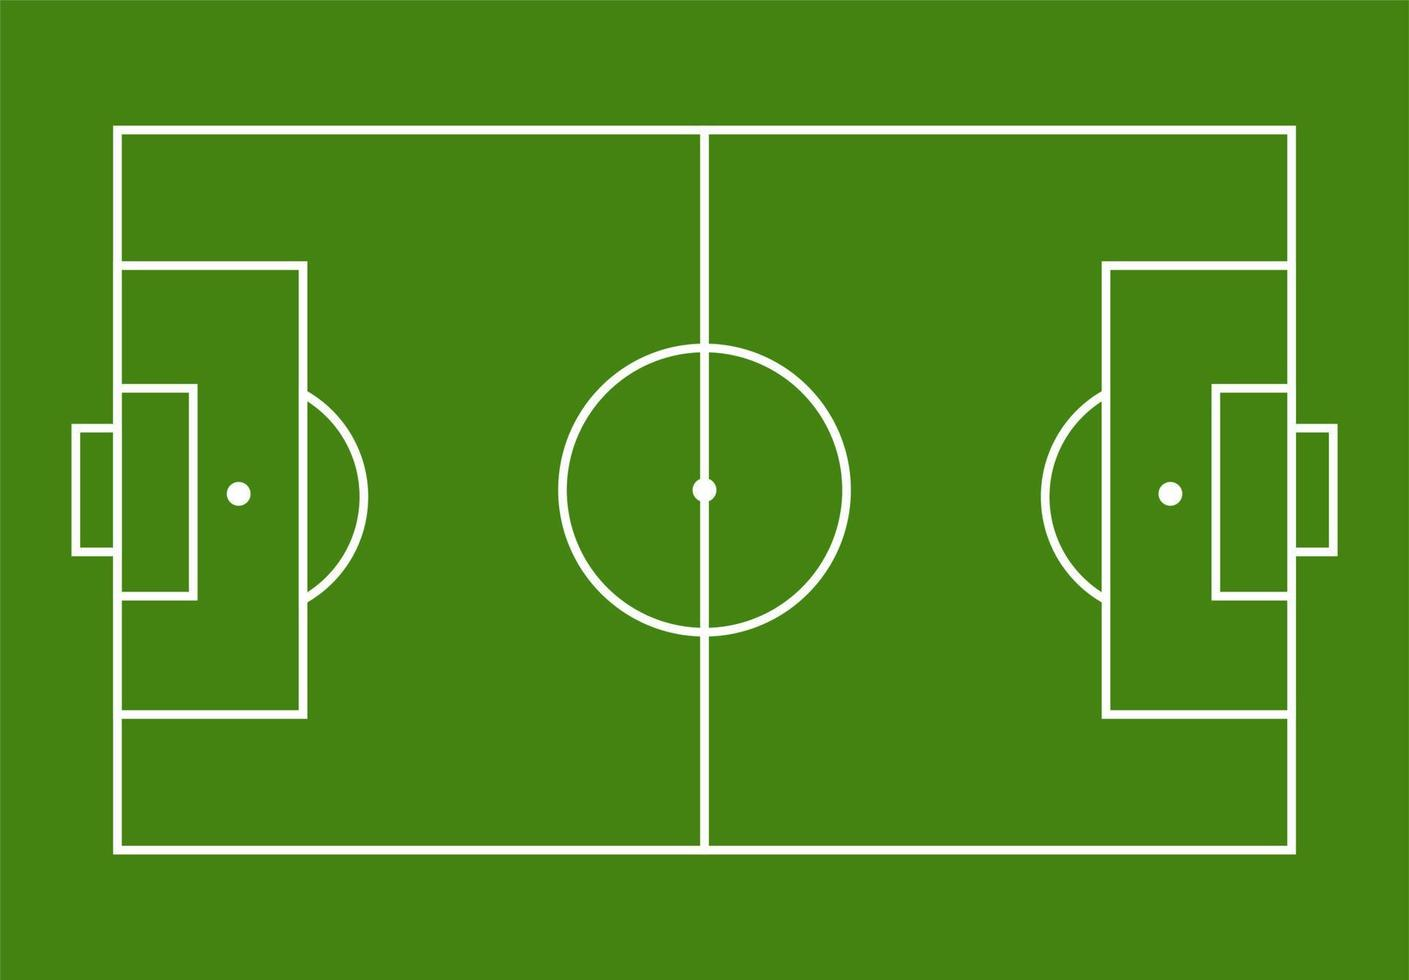
\includegraphics[width=0.75\textwidth]{figures/campo_futbol_vecteezy.jpg}
\caption{Campo de fútbol estándar visto en planta \citep{vecteezy2026campo}. Las
medidas FIFA reglamentarias empleadas como referencia para la homografía y
para los mapas de calor de este proyecto
(sección~\ref{sec:implementacion-metadatos}) son: 105\,m $\times$ 68\,m de
terreno de juego, área grande 16{,}5\,m $\times$ 40{,}3\,m, área pequeña
5{,}5\,m $\times$ 18{,}3\,m, círculo central de 9{,}15\,m de radio.}
\label{fig:fundamentos-campo}
\end{figure}

Esa transformación, cuando la cámara se puede aproximar como una
proyección perspectiva pura sobre un plano. El terreno de juego es, a
efectos prácticos, plano, se describe matemáticamente mediante una
\textbf{homografía}: una matriz $H$ de $3\times 3$ que relaciona las
coordenadas homogéneas de un punto en el plano imagen,
$\mathbf{p} = (x, y, 1)^\top$, con las coordenadas homogéneas del punto
correspondiente en el plano del campo, $\mathbf{p}' = (x', y', 1)^\top$,
mediante

\begin{equation}
\mathbf{p}' \sim H\,\mathbf{p},
\label{eq:fundamentos-homografia}
\end{equation}

donde $\sim$ indica igualdad salvo un factor de escala, propio de las
coordenadas homogéneas \citep{opencv2026homography}. La matriz $H$ tiene 8
grados de libertad (9 elementos menos 1 por el factor de escala libre), por
lo que puede calcularse de forma exacta a partir de 4 pares de puntos
correspondientes conocidos (un punto en la imagen y su posición real
equivalente en el campo) mediante un sistema de ecuaciones lineales;
disponer de más de 4 correspondencias permite, además, calcular $H$ por
mínimos cuadrados y obtener una estimación más robusta frente a errores de
medición en los puntos de referencia.

\begin{figure}[htp]
\centering
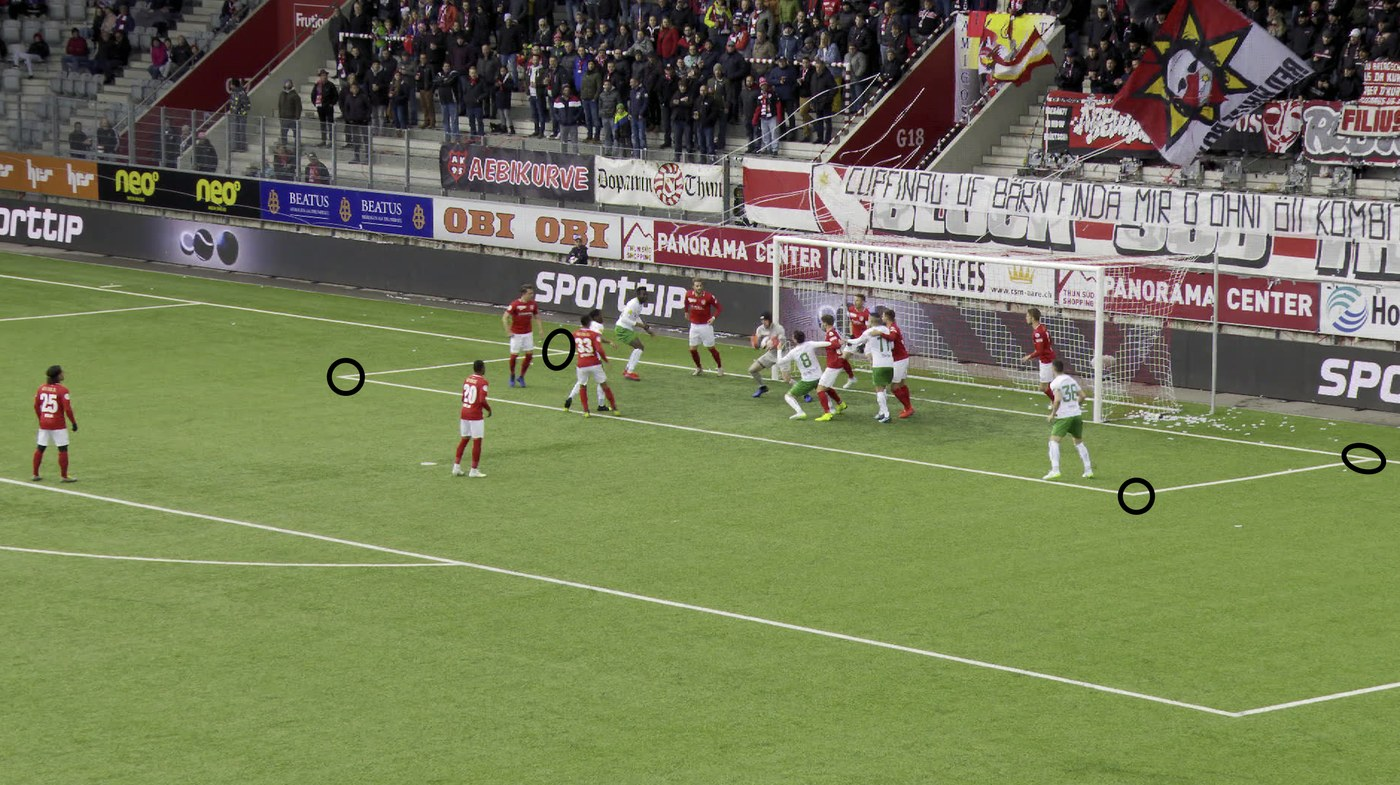
\includegraphics[width=0.92\textwidth]{figures/homografia-real.jpg}
\caption{Puntos de referencia marcados sobre un frame real de
retransmisión, usados para calcular la homografía: las cuatro esquinas
del área pequeña, cuyas coordenadas de campo son conocidas por las
medidas FIFA (Figura~\ref{fig:fundamentos-campo}).}
\label{fig:fundamentos-homografia-ejemplo}
\end{figure}

En un escenario ideal, en el que la cámara de retransmisión permaneciera
completamente fija durante todo el partido, bastaría con calcular $H$ una
única vez, identificando manualmente 4 puntos de referencia reconocibles en
el campo, por ejemplo, las esquinas del área pequeña, cuyas medidas FIFA
son conocidas y fijas (5{,}5\,m $\times$ 18{,}3\,m,
Figura~\ref{fig:fundamentos-campo}) y sus coordenadas de píxel
correspondientes en un frame representativo. Esta es, de hecho, la
aproximación seguida en este proyecto, pero limitada deliberadamente a
tramos concretos de vídeo con cámara estable, dado que las cámaras de
retransmisión real de SoccerNet se mueven de forma continua (paneos,
zooms) a lo largo de toda la secuencia (lo que exigiría recalcular $H$
de forma dinámica, frame a frame, un problema de calibración de cámara
considerablemente más complejo y fuera del alcance de este proyecto). Las
implicaciones prácticas de esta limitación, y la alternativa de proyección
aproximada empleada para el resto del dataset, se detallan en la
sección~\ref{sec:implementacion-homografia}.

\section{Trabajos relacionados y posicionamiento de este TFG}
\label{sec:fundamentos-relacionados}

El propio ecosistema SoccerNet organiza, además del dataset, un reto anual
de seguimiento multiobjeto (\emph{SoccerNet Player Tracking Challenge}) con
un servidor de evaluación público y un \emph{leaderboard} de equipos
participantes, lo que ofrece el punto de comparación más directo y
verificable para situar los resultados de este proyecto frente al estado
del arte práctico.

La edición 2023 del reto \citep{cioppa2023soccernetchallenges}, con 7 equipos
y 83 envíos, resulta muy informativa sobre qué enfoques resultan
competitivos en la práctica: el equipo ganador (Kalisteo) alcanzó
HOTA\,=\,75{,}61 combinando un detector YOLO-X afinado con un tracker
propio basado en el algoritmo húngaro
y un filtro de Kalman con compensación de movimiento de cámara; y, de forma especialmente
relevante para las decisiones de este proyecto, varios de los equipos
mejor clasificados construyeron su solución precisamente sobre
\textbf{ByteTrack} o la familia \textbf{SORT/OC-SORT}, por ejemplo, SAIVA Tracking
sobre ByteTrack, ZTrackers sobre YOLOv5 combinado con ByteTrack, y
MOT4MOT sobre DeepOCSORT, lo que confirma que ambos algoritmos
constituyen una base representativa y competitiva del estado del arte
práctico.

El HOTA integrado en test obtenido en este proyecto
con OC-SORT (75{,}43), resulta muy próximo al del equipo ganador del
reto oficial 2023 (75{,}61) aunque a partir de una posición menos favorable
en dos aspectos: sin ningún entrenamiento ni ajuste de detector
específico para fútbol, y con los algoritmos de tracking en su
configuración por defecto para esa comparación concreta. No se trata, por
tanto, de una comparación totalmente equivalente ni se trata de un intento
de superar el estado del arte del reto, es una referencia
que sitúa los resultados de este TFG en un rango realista y defendible
frente a soluciones desarrolladas específicamente para competir.

Este proyecto no busca competir en ese \emph{leaderboard}, sino dos objetivos distintos que
el reto no cubre: una comparación rigurosa entre dos algoritmos clásicos de
\emph{tracking-by-detection} bajo las mismas condiciones mi. Y segundo, la construcción de un pipeline
completo de extracción de metadatos deportivos y la
exposición des sus resultados en una aplicación web, que va
más allá de la propia tarea de tracking en la que se detiene el reto
oficial.

